\begin{doubledpage}{theorem}{Brook's theorem \cite{brooks1941colouring}}{ 
  Let $G$ be a connected graph which is not an odd cycle or a complete graph. Then $\gamma(G)\leq \Delta(G)$. \label{emb:thm:brooks}}


The basic observation in this proof is that you can switch two colors in a graph coloring and still wind up with a valid graph coloring. 

 We induct on the number of vertices. The base case is to look at the trivial graph, and it follows trivially. 

  Now for the inductive step, assume that $G\setminus v$ satisfies the theorem by induction hypothesis. If $v$ has degree less than $\Delta(G)$, then we can color it greedily; therefore we should assume that $v$ is a vertex of degree $\Delta(G)$. We may also make the assumption that the neighbors of $v$ do not make a complete graph. 
  
  Given a coloring of $G\setminus v$, we get a $\Delta(G)$-coloring of $G$. We now have 2 cases:

 \textbf{Case 1:} Suppose that 2 of the neighbors of $v$ are colored with the same color. Then not all $\Delta(G)$-colors are used in $N(v)$, so we may color $v$ with the remaining color. 
 
 \textbf{Case 2:} We are now in the harder case, where $N(v)$ is uses every color. We therefore may index the points in the neighborhood of $v$ by the color set: with this labeling, $N(v)=\{v_1, \ldots, v_\Delta\}$. We want to show that we can simplify this coloring. For our construction,  $H_{i,j}$ be the subgraph of $G\setminus v$ which has been colored by $i$ and $j$. Here are some simple cases that we can rule out: 
 
\begin{paragraphfigureenv}{191figures/topgraph_colordegree1.tikz}
\textbf{Easy Case:}Suppose that for some $i, j$, $v_i$ and $v_j$ do not lie in the same connected component of $H_{i,j}$. Then let $C^i_{i,j}$ be the connected component of $H_{i,j}$ containing $v_i$. On this subgraph, switch the colors of $i$ and $j$. Now this produces a valid coloring on $G\setminus v$, and the vertex $v_i$ will now be colored $j$. Now we can color the vertex $v$ the color $i$.  
\end{paragraphfigureenv}


\begin{paragraphfigureenv}{191figures/topgraph_colordegree2.tikz}
\textbf{Easy Case:} Additionally, we may assume that the connected component containing $v_i$ and $v_j$ is a path. If it wasn't a path, then there is a vertex $w$ that has degree 3 in the path. Necessarily, one of $N(w)$ is not colored with $i$, $j$ or some other color $k$. Color $w$ with the color $k$ instead. With this updated coloring, we have that $H_{ij}$ separates the vertices $v_i$ and $v_j$, and we may apply the previous easy case. 
\end{paragraphfigureenv}


\begin{paragraphfigureenv}{191figures/topgraph_colordegree3.tikz}
  \textbf{Ease Case:} For any $i, j, k$, the paths we've constructed from $v_i$ to $v_j$ and from $v_j$ to $v_k$ may only intersect at $v_j$. Any other intersection point $w$ would have two neighbors colored $i$, and two neighbors colored $k$, and could therefore be colored some other 4th color
\end{paragraphfigureenv}


Since the neighbors of $v$ do not make a complete graph, we can assume without loss of generality that $v_1v_2$ is not an edge of $G$.  Let $P_{12}$ be the path from $v_1$ to $v_2$. 
Let $w$ be a point on that path closest to $v_1$ (this point will be colored $2$. ) \\
We now will generate a new coloring for $G$ by switching colors 1 and 3 in the path from $v_1$ to $v_3$. I'll label the changed color vertices with parenthesis. Take a look at Figure \ref{fig:brooks} for pictures.

\begin{figure}[h]
  \newcommand{\vertexradius}{2.5pt}
\newcommand{\vertexscale}{.5}
\newcommand{\bigvertexscale}{1}
\newcommand{\vertex}{\node[circle, fill=black, scale=\vertexscale] }
\newcommand{\highlighta}{red!20}
\newcommand{\highlightb}{blue!20}
\newcommand{\highlightc}{green!20}
\newcommand{\shadinga}{gray!20}
\newcommand{\smallvertex}{\node[circle, fill=black, scale=.2]}
\newcommand{\highlightlinewidth}{3pt}

\tikzset{every path/.style={line width=1 pt}}
\centering
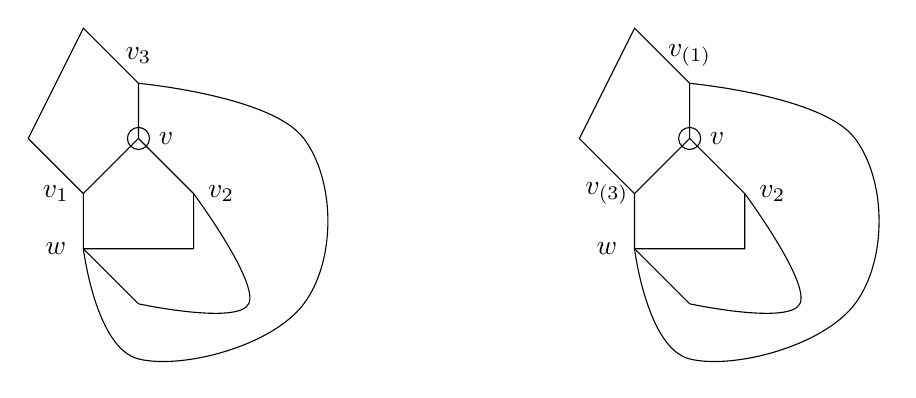
\begin{tikzpicture}[scale=.7]

\draw (5,0) circle[radius=.2];

\draw (5,0) -- (4,-1) -- (3,0) -- (4,2) -- (5,1) -- (5,0);
\draw (4,-1) -- (4,-2) -- (6,-2) -- (6,-1) -- (5,0);


\draw (-5,0) -- (-6,-1) -- (-7,0) -- (-6,2) -- (-5,1) -- (-5,0);
\draw (-6,-1) -- (-6,-2) -- (-4,-2) -- (-4,-1) -- (-5,0);
\draw (-6,-2) -- (-5,-3);
\draw  plot[smooth, tension=.7] coordinates {(-5,-3) (-3,-3) (-4,-1)};
\draw (4,-2) -- (5,-3);
\draw  plot[smooth, tension=.7] coordinates {(5,-3) (7,-3) (6,-1)};
\draw  plot[smooth, tension=.7] coordinates {(4,-2) (5,-4) (8,-3) (8,0) (5,1)};
\draw  plot[smooth, tension=.7] coordinates {(-6,-2) (-5,-4) (-2,-3) (-2,0) (-5,1)};
\node at (-6.5,-1) {$v_1$};
\node at (-6.5,-2) {$w$};
\node at (-5,1.5) {$v_3$};
\node at (-3.5,-1) {$v_2$};
\node at (-4.5,0) {$v$};
\node at (3.5,-1) {$v_{(3)}$};
\node at (3.5,-2) {$w$};
\node at (5.5,0) {$v$};
\node at (5,1.5) {$v_{(1)}$};
\node at (6.5,-1) {$v_2$};\vertexc at (4,2) {};
\vertexb at (4,-2) {};
\vertexa at (3,0) {};
\vertexa at (6,-2) {};
\vertexa at (5,1) {};
\vertexb at (6,-1) {};
\vertexc at (4,-1) {};
\vertexc at (5,-3) {};
\vertexc at (-5,-3) {};
\vertexa at (-6,2) {};
\vertexb at (-6,-2) {};
\vertexc at (-7,0) {};
\vertexa at (-4,-2) {};
\vertexc at (-5,1) {};
\vertexb at (-4,-1) {};
\vertexa at (-6,-1) {};
\draw (-5,0) circle[radius=.2];
\end{tikzpicture}
\caption{Recoloring path segment to simplify the coloring.}
\label{fig:brooks}
\end{figure}
With this new set-up $w$ is in the connected component from $v_1=v_{(3)}$ to $v_2$, and is still colored 2.\\
In this new coloring look at the $\{1, 2\}$ colored path between $v_2$ and $v_{(1)}$ The vertex $w$ must belong to this new path. Since $w\in N(v_{(3)})$, we must additionally also have that $w$ is in the $\{2, 3\}$ colored path between $v_{(3)}$ and $v_2$. \\
This means that $u$ belongs to 2 paths. This means that we are in the 3rd kind of easy case, and we can simplify our coloring. 
 


\end{doubledpage}